
\section{Preliminary}



\subsection{Maximal Update Parametrization (\texorpdfstring{$\boldsymbol{\mu}$}{mu}P) }
\label{sec:bg_mup}

$\boldsymbol{\mu}$P prescribes how
activations and weight updates should scale with width to preserve feature learning~\citep{yang2023spectral}.
Ideal feature learning requires the scale of activations to remain as invariant as possible.
We use \textbf{operator norm} to characterize how the norm of activations changes through a linear layer.

Considering a linear layer $\vy=\mW\vx$ with
$\mW\in\mathbb{R}^{d_{\mathrm{out}}\times d_{\mathrm{in}}},\vx\in\mathbb{R}^{d_{\mathrm{in}}}$, the RMS norm is defined as
\begin{equation}
\|\vx\|_{\mathrm{rms}} := \frac{\|\vx\|_2}{\sqrt{d_{\mathrm{in}}}},
\end{equation}
while the RMS-to-RMS operator norm is defined as
\begin{equation}
\|\mW\|_{\mathrm{rms}\to\mathrm{rms}}
:= \sup_{\vx\neq\bm{0}}
\frac{\|\mW\vx\|_{\mathrm{rms}}}{\|\vx\|_{\mathrm{rms}}}.
\label{eq:rms_to_rms}
\end{equation}


$\boldsymbol{\mu}$P scale invariance requires maintaining
$\|\vy\|_{\mathrm{rms}}=\|\vx\|_{\mathrm{rms}}=\Theta(1),$
which is equivalent to enforcing the RMS-to-RMS condition
$\|\mW\|_{\mathrm{rms}\to\mathrm{rms}}= \|\mW\|_2\sqrt{{d_{\mathrm{in}}}/{d_{\mathrm{out}}}}=\Theta(1).$
This induces the following spectral norm constraint on the weight matrix
$
\|\mW\|_2 = \Theta (\sqrt{{d_{\mathrm{out}}}/{d_{\mathrm{in}}}}).
$
A similar requirement applies to parameter updates; together, we refer to these as the spectral $\boldsymbol{\mu}$P condition below.


\begin{mdframed}[style=MyBoxStyle1, frametitle={Spectral $\boldsymbol{\mu}$P Condition}, nobreak=true]
\citet{yang2023spectral} shows that preserving \emph{scale-invariant activations} for feature learning requires the same law to hold for both weights and their updates:
\[
\|\mW\|_2 = \Theta\left(\sqrt{\frac{d_{\mathrm{out}}}{d_{\mathrm{in}}}}\right),
\qquad
\|\mPhi\|_2 = \Theta\left(\sqrt{\frac{d_{\mathrm{out}}}{d_{\mathrm{in}}}}\right).
\]
\end{mdframed}



\subsection{Steepest Descent under Different Norms}
\label{sec:bg_mdl}

Following~\citet{bernstein2024oldoptimizernewnorm, cesista2025sdcbs}, many successful optimizers can be interpreted as \textbf{first-order} methods without convexity assumptions. Specifically, after switching off exponential moving averages, these algorithms reduce to instances of steepest descent governed by distinct norms:  SGD corresponds to the Frobenius norm $\|\!\cdot\!\|_F$, AdamW~\citep{loshchilov2019decoupled} to the $\ell_{\infty}$ norm, and Shampoo~\citep{gupta2018shampoo} to the spectral norm $\|\!\cdot\!\|_2$.

In this view, we determine the update $\mPhi$ by iteratively minimizing a first-order Taylor approximation of the loss around the current weights $\mW$, subject to a hard constraint on the step size:
\begin{equation}
    \mPhi := \underset{\|\mPhi\| \le \eta}{\argmin} \left\{ \mathcal{L}(\mW) + \left\langle \nabla_\mW\mathcal{L}(\mW), \mPhi \right\rangle \right\} = \underset{\|\mPhi\| \le \eta}{\argmin} \langle \mG, \mPhi \rangle,
    \label{eq:constrained_opt}
\end{equation}
where $\mG:=\nabla_\mW\mathcal{L}(\mW)$ is the gradient of the loss function at $\mW$. The update is thus determined by two priors: a \textbf{norm} $\|\!\cdot\!\|$ assigned according to the specific \emph{functional role} of the module, and a \textbf{step size} $\eta$ that governs the update scale. The solution is as follows:

\begin{mdframed}[style=MyBoxStyle1, frametitle={Definition 1: Steepest Descent Update}, nobreak=true]

Given a norm $\|\!\cdot\!\|$ defining the geometry and a step size $\eta$ governing the scale, the \textbf{steepest descent update} solution to \cref{eq:constrained_opt} is given by
\begin{equation}
    \mPhi = -\eta \cdot \mPhi_{\text{unit}},
\quad
\text{where}
\quad
\mPhi_{\text{unit}} := \underset{\|\mT\| \leq 1}{\arg\max} \langle \mG, \mT \rangle,
\end{equation}
\end{mdframed}


% \subsection{Steepest Descent under Different Norms}
% \label{sec:bg_mdl}

% Following metrized deep learning~\citep{bernstein2024oldoptimizernewnorm}, many successful optimizers (e.g. AdamW~\citep{loshchilov2019decoupled}, Shampoo~\citep{gupta2018shampoo}, Prodigy~\citep{mishchenko2024prodigy}) can be interpreted as \textbf{first-order} methods without convexity assumptions. Specifically, after switching off exponential moving averages, these algorithms reduce to instances of steepest descent governed by distinct norms. Under this framework, an optimizer is fundamentally defined by a weight update $\mPhi$ that minimizes a quadratic model of the loss:
% \begin{equation}
%     \mPhi := \underset{\mPhi}{\argmin} \left\{ \mathcal{L}(\mW) + \langle \mG, \mPhi \rangle + \frac{\lambda}{2} \|\mPhi\|^2 \right\}.
%     \label{eq:quadratic}
% \end{equation}

% The update is thus determined by two priors: a \textbf{norm} $\|\!\cdot\!\|$ assigned according to the specific \emph{functional role} of the module, and a \textbf{sharpness} $\lambda$ that governs the update scale. The solution is as follows:

% \begin{mdframed}[style=MyBoxStyle1, frametitle={Definition 1: Steepest Descent Update}, nobreak=true]

% Given a norm $\|\!\cdot\!\|$ that endows the parameter space with a geometry, the \textbf{steepest descent update} is
% \begin{equation}
%   \mPhi = -\eta \cdot \mPhi_{\text{unit}},
% \quad
% \text{where}
% \quad
% \mPhi_{\text{unit}} := \underset{\|\mT\| \leq 1}{\arg\max} \langle \mG, \mT \rangle,
% \quad
% \text{and}
% \quad
% \eta := \frac{\|\mG\|_\dagger}{\lambda}.
% \label{eq:dual_form}
% \end{equation}
% Here, $\|\mG\|_\dagger := \max_{\|\mT\| \leq 1} \langle \mG, \mT \rangle$ is the \textbf{dual norm} of the gradient $\mG$ induced by $\|\!\cdot\!\|$.
% \end{mdframed}
% This perspective unifies diverse algorithms by mapping them to their underlying geometries: SGD corresponds to Frobenius norm $\|\!\cdot\!\|_F$, Adam to $l_{\infty}$ norm, and Shampoo to spectral norm $\|\!\cdot\!\|_2$.


\subsection{Muon Optimizer}
\label{sec:bg_spectral_sd}

Following the framework of metrized deep learning (\cref{sec:bg_mdl}), Muon~\citep{jordan2024muon} can be interpreted as steepest descent under the \textbf{spectral norm}. For a 2D weight matrix $\mW$, the spectral norm $\|\!\cdot\!\|_2$ \footnote{For vectors, $\| \vv\|_2$ denotes the $\ell_2$ norm; for matrices, $\|\mW\|_2 $ denotes the (induced $\ell_2\!\to\!\ell_2$) spectral norm.}
 gives the tightest bound on the matrix's input-output gain:
\begin{equation}
\|\mW\|_2 := \sup_{\vx\ne\bm{0}} \frac{\|\mW \vx\|_2}{\|\vx\|_2},
\end{equation}
By choosing the spectral norm to constrain the update direction $\mPhi$, the steepest descent direction is uniquely given by the \textbf{matrix sign function (msign)} (\cref{app:dual}):
\begin{equation}
\operatorname{msign}(\mG) = \mU \operatorname{sign}(\boldsymbol{\Sigma}) \mV^\top
= \mU_{[:, :r]} \mV_{[:, :r]}^\top,
\end{equation}
where $\mG = \mU \boldsymbol{\Sigma} \mV^\top$ is the singular value decomposition (SVD). The msign operation orthogonalizes the gradient, equalizing all active singular directions and yielding a spectrum isotropic update. A key contribution of Muon is the efficient approximation of $\operatorname{msign}(\mG)$ via Newton–Schulz iterations which can be implemented on GPUs.

However, Muon constrains only the backward update $\mPhi$, leaving the forward weights $\mW$ unconstrained. This often leads to unstable $\boldsymbol{\mu}$P feature learning in hidden states rms, motivating our development of \textbf{a fully aligned approach that constrains both $\mW$ and $\mPhi$}.

\begin{figure}[H]%DONOTCHANGE
    \centering
    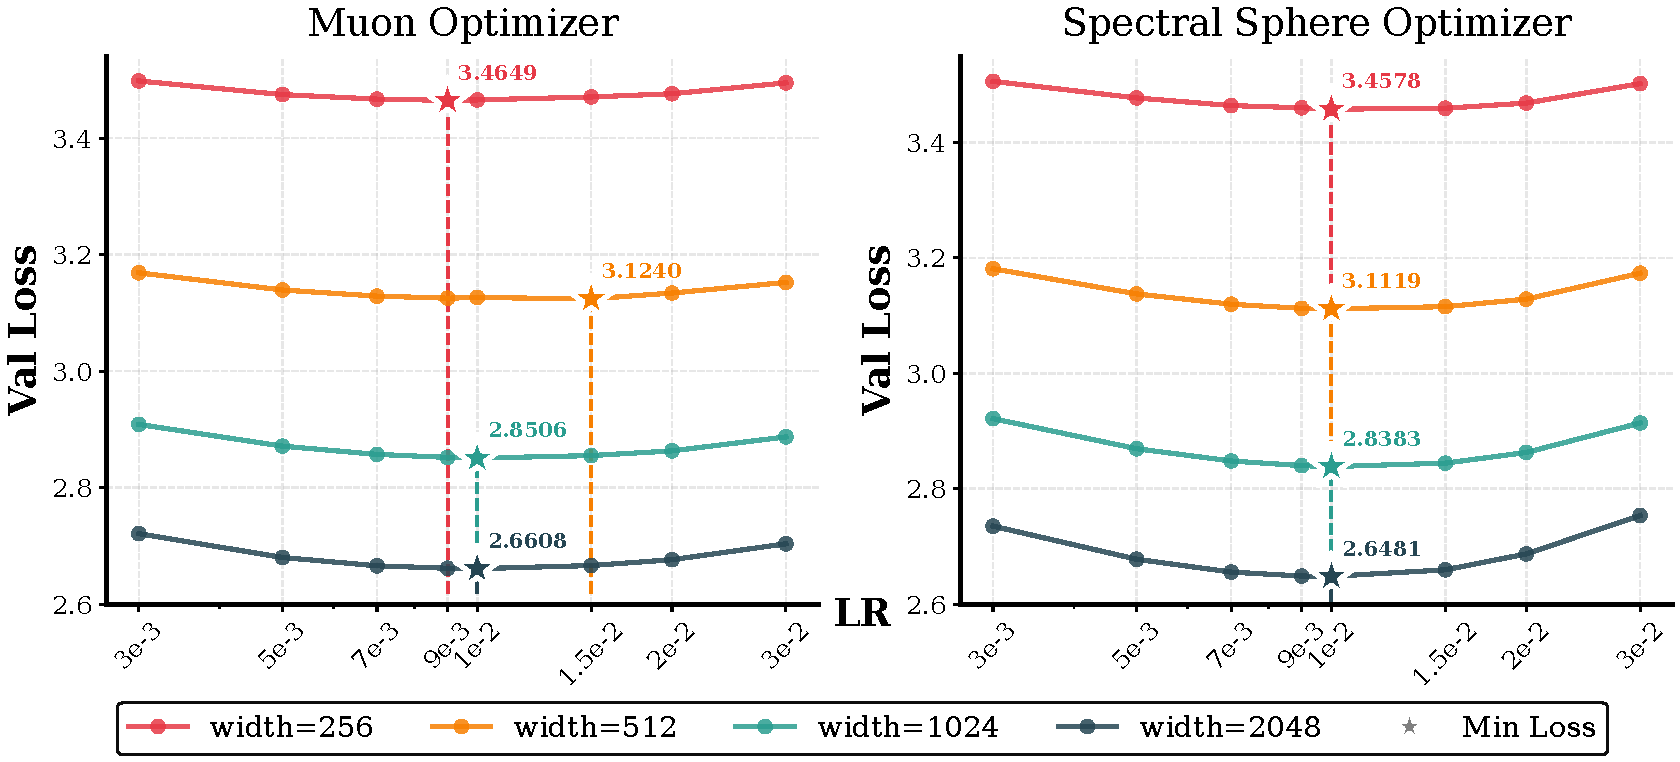
\includegraphics[width=0.85\linewidth]{figures/mup_comparison.pdf}
    \caption{
    \textbf{$\boldsymbol{\mu}$P width scaling across 25$\times$ model sizes (70M to 1.8B).}
    Although $\boldsymbol{\mu}$P aims for width-invariant scaling, \textcolor{MuonColor}{Muon} still exhibits notable optimal learning rate drift. In contrast, our \textcolor{SpectralSphereColor}{Spectral Sphere} achieves stable LR transfer, while also obtaining \textbf{lower optimal loss than} \textcolor{MuonColor}{Muon}. More details and related experiments are provided in~\cref{app:mup_width}.
    }
    \label{fig:mup_width}
\end{figure}
